\section{Abgeleiteten Klassen}
\subsection{Speicheranordnung}
Die Strukturen in C sind sensitiv zur Reihenfolge der Variablen.

%\begin{minted}{C}
%  typedef struct base_t {
%    int a;
%    int b;
%  } base_t;

%  typedef struct derived_t {
%    base_t super;
%    double a;
%    double b;
%  } derived_t;
%\end{minted}

\inputminted{c}{code/structlayout/base.c}
\inputminted{c}{code/structlayout/derived.c}
\inputminted{c}{code/structlayout/cast.c}


\begin{figure}[h]
	\centering
	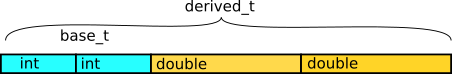
\includegraphics[width=0.8\textwidth]{layout.png}
	\caption{Datalayout}
	\label{fig:datalayout}
\end{figure}


\subsection{Virtuelle Tabelle}
Die virtuelle Tabelle beinhaltet Funktionspointer.

Die Abgeleitee Klasse kann eine Funktion reimplementieren, z.B. die Funktion \mintinline{c}{print} kann bei einem Angestellten nur den Vornamen und Nachnamen ausgeben.
Die abgeleitet Klasse kann aber zusätzliche Parameter beinhalten, die wir ebenfalls ausgeben möchten.
Deshalb wollten wir eine andere Funktion, mit einer identischer Signatur benutzen, benutzen, die uns eine andere, passende Ausgabe macht.


Die virtuelle Tabelle ist ein


\begin{code}
	\caption{Basis Klasse}
	\label{code:vtbl:base}
	\inputminted{cpp}{code/virt_table/employee.c}
\end{code}


\begin{code}
	\caption{Abgeleitete Klasse}
	\label{code:vtbl:derived}
	\inputminted{cpp}{code/virt_table/manager.c}
\end{code}



\begin{code}
	\caption{Abgeleitete Klasse}
	\label{code:vtbl:call}
	\inputminted{cpp}{code/virt_table/call.c}
\end{code}

\subsection{Beispiel}
Die Grundidee der Vererbung ist die Wiederverwendung vom Code.
Dadurch wird auch die Wartung der Programme erheblich vereinfacht.
Nach der Vererbung erhält die abgeleitete Klasse die Funktionalität der Basisklasse.

Den Preis, den wir dafür bezahlen, ist typischerweise den Speicher für ein Zeiger auf eine virtuelle Tabelle (8 bytes in der 64bit-Architektur).
Das ist aber eine Implementierungssache und der Preis kann bei anderen Implementierungen ganz anders sein.


\begin{code}
	\inputminted{cpp}{code/employees_virt/employee.h}
\end{code}

\begin{code}
	\inputminted{cpp}{code/employees_virt/employee.c}
\end{code}


%\begin{code}
%  \inputminted{cpp}{code/employees_virt_cpp/main.cpp}
%  \inputminted[bgcolor=white]{text}{code/employees_virt_cpp/output.txt}
%\end{code}

%\begin{code}
%  \caption{main}
%  \inputminted{c}{code/employees_virt/main.c}
%  \inputminted[bgcolor=white]{text}{code/employees_virt/output.txt}
%\end{code}
